\documentclass{standalone}
\usepackage{tikz}
\usetikzlibrary{patterns, positioning}
\usepackage[sfdefault]{ClearSans} %% option 'sfdefault' activates Clear Sans as the default text font
\usepackage[T1]{fontenc}

\begin{document}
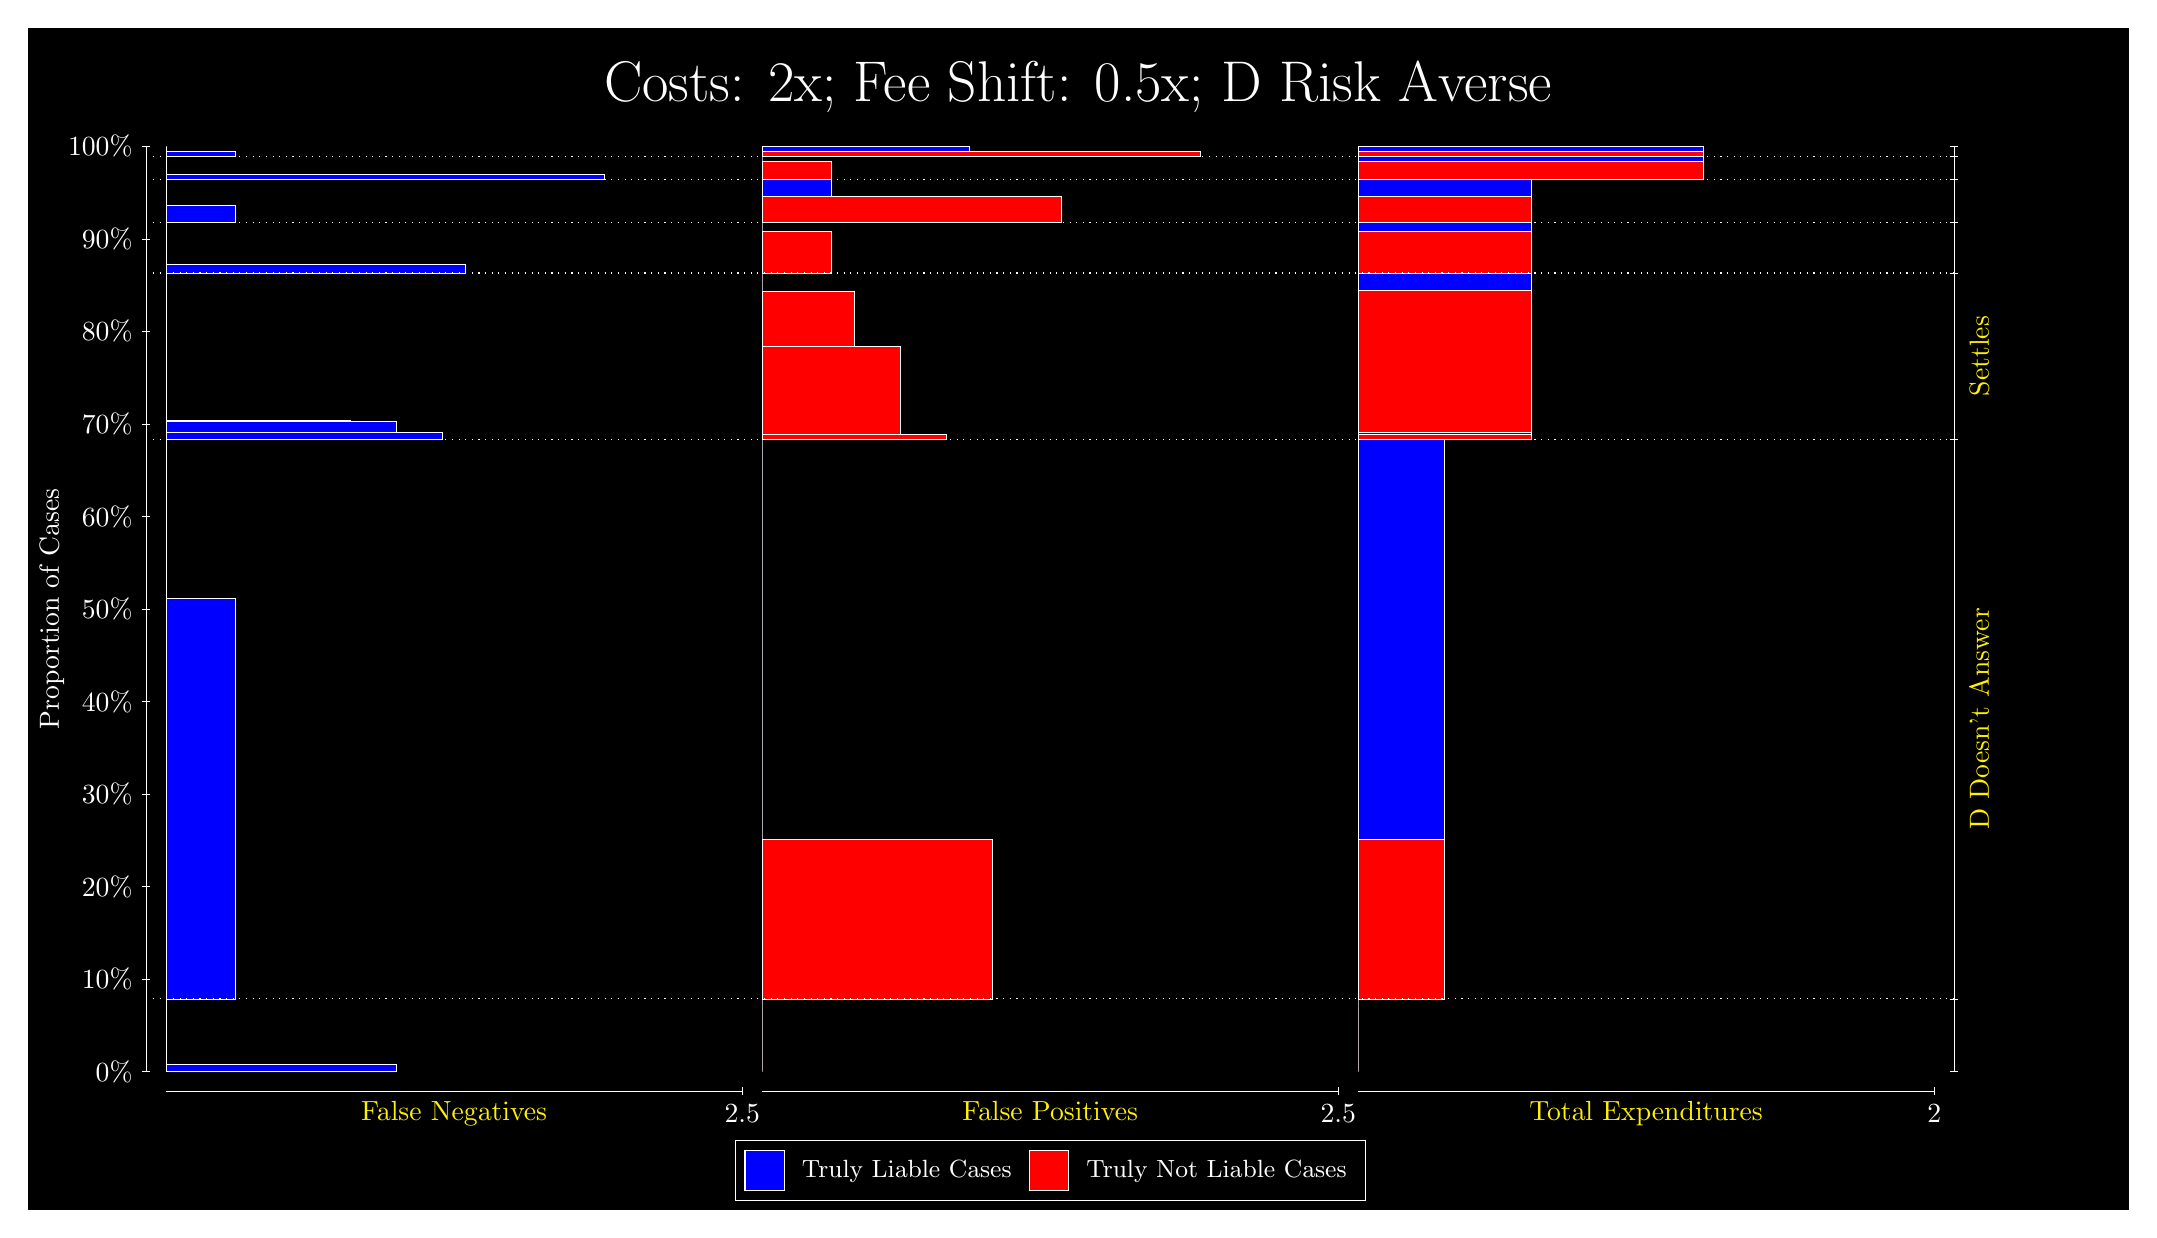
\begin{tikzpicture}
\draw[fill=black] (0,0) rectangle (26.667,15);
\draw[text=white] (0,13.5) rectangle (26.667,15) node[midway] {\huge Costs: 2x; Fee Shift: 0.5x; D Risk Averse};
\draw[white, very thin] (1.5,1.75) -- (1.5,13.5);
\node[rotate=90, text=white, anchor=center] at (0.3, 7.625) {Proportion of Cases};
\draw[white, very thin] (1.45,1.75) -- (1.55,1.75);
\node[text=white, anchor=east] at (1.45, 1.75) {0\%};
\draw[white, very thin] (1.45,2.925) -- (1.55,2.925);
\node[text=white, anchor=east] at (1.45, 2.925) {10\%};
\draw[white, very thin] (1.45,4.1) -- (1.55,4.1);
\node[text=white, anchor=east] at (1.45, 4.1) {20\%};
\draw[white, very thin] (1.45,5.275) -- (1.55,5.275);
\node[text=white, anchor=east] at (1.45, 5.275) {30\%};
\draw[white, very thin] (1.45,6.45) -- (1.55,6.45);
\node[text=white, anchor=east] at (1.45, 6.45) {40\%};
\draw[white, very thin] (1.45,7.625) -- (1.55,7.625);
\node[text=white, anchor=east] at (1.45, 7.625) {50\%};
\draw[white, very thin] (1.45,8.8) -- (1.55,8.8);
\node[text=white, anchor=east] at (1.45, 8.8) {60\%};
\draw[white, very thin] (1.45,9.975) -- (1.55,9.975);
\node[text=white, anchor=east] at (1.45, 9.975) {70\%};
\draw[white, very thin] (1.45,11.15) -- (1.55,11.15);
\node[text=white, anchor=east] at (1.45, 11.15) {80\%};
\draw[white, very thin] (1.45,12.325) -- (1.55,12.325);
\node[text=white, anchor=east] at (1.45, 12.325) {90\%};
\draw[white, very thin] (1.45,13.5) -- (1.55,13.5);
\node[text=white, anchor=east] at (1.45, 13.5) {100\%};

\draw[white, very thin] (24.457,1.75) -- (24.457,13.5);
\draw[white, very thin] (24.407,1.75) -- (24.507,1.75);
\node[anchor=west] at (24.407, 1.75) {};
\draw[white, very thin] (24.407,2.6725) -- (24.507,2.6725);
\node[anchor=west] at (24.407, 2.6725) {};
\draw[white, very thin] (24.407,9.7811) -- (24.507,9.7811);
\node[anchor=west] at (24.407, 9.7811) {};
\draw[white, very thin] (24.407,11.891) -- (24.507,11.891);
\node[anchor=west] at (24.407, 11.891) {};
\draw[white, very thin] (24.407,12.538) -- (24.507,12.538);
\node[anchor=west] at (24.407, 12.538) {};
\draw[white, very thin] (24.407,13.08) -- (24.507,13.08);
\node[anchor=west] at (24.407, 13.08) {};
\draw[white, very thin] (24.407,13.373) -- (24.507,13.373);
\node[anchor=west] at (24.407, 13.373) {};
\draw[white, very thin] (24.407,13.5) -- (24.507,13.5);
\node[anchor=west] at (24.407, 13.5) {};

\draw[white, very thin, fill=blue] (1.75,1.75) rectangle (4.6775,1.8471);
\draw[white, very thin, fill=red] (1.75,1.8471) rectangle (1.75,2.6725);
\draw[white, very thin, fill=blue] (1.75,2.6725) rectangle (2.6283,7.7542);
\draw[white, very thin, fill=red] (1.75,7.7542) rectangle (1.75,9.7811);
\draw[white, very thin, fill=blue] (1.75,9.7811) rectangle (5.2631,9.8661);
\draw[white, very thin, fill=blue] (1.75,9.8661) rectangle (4.6775,10.002);
\draw[white, very thin, fill=blue] (1.75,10.002) rectangle (4.092,10.019);
\draw[white, very thin, fill=red] (1.75,10.019) rectangle (1.75,11.891);
\draw[white, very thin, fill=blue] (1.75,11.891) rectangle (5.5558,12.006);
\draw[white, very thin, fill=red] (1.75,12.006) rectangle (1.75,12.538);
\draw[white, very thin, fill=blue] (1.75,12.538) rectangle (2.6283,12.754);
\draw[white, very thin, fill=red] (1.75,12.754) rectangle (1.75,13.08);
\draw[white, very thin, fill=blue] (1.75,13.08) rectangle (7.3123,13.141);
\draw[white, very thin, fill=red] (1.75,13.141) rectangle (1.75,13.373);
\draw[white, very thin, fill=blue] (1.75,13.373) rectangle (2.6283,13.44);
\draw[white, very thin, fill=red] (1.75,13.44) rectangle (1.75,13.5);
\draw[white, very thin, fill=red] (9.3189,1.75) rectangle (9.3189,2.5754);
\draw[white, very thin, fill=blue] (9.3189,2.5754) rectangle (9.3189,2.6725);
\draw[white, very thin, fill=red] (9.3189,2.6725) rectangle (12.246,4.6994);
\draw[white, very thin, fill=blue] (9.3189,4.6994) rectangle (9.3189,9.7811);
\draw[white, very thin, fill=red] (9.3189,9.7811) rectangle (11.661,9.8455);
\draw[white, very thin, fill=red] (9.3189,9.8455) rectangle (11.075,10.961);
\draw[white, very thin, fill=red] (9.3189,10.961) rectangle (10.49,11.654);
\draw[white, very thin, fill=blue] (9.3189,11.654) rectangle (9.3189,11.891);
\draw[white, very thin, fill=red] (9.3189,11.891) rectangle (10.197,12.423);
\draw[white, very thin, fill=blue] (9.3189,12.423) rectangle (9.3189,12.538);
\draw[white, very thin, fill=red] (9.3189,12.538) rectangle (13.125,12.864);
\draw[white, very thin, fill=blue] (9.3189,12.864) rectangle (10.197,13.08);
\draw[white, very thin, fill=red] (9.3189,13.08) rectangle (10.197,13.312);
\draw[white, very thin, fill=blue] (9.3189,13.312) rectangle (9.3189,13.373);
\draw[white, very thin, fill=red] (9.3189,13.373) rectangle (14.881,13.433);
\draw[white, very thin, fill=blue] (9.3189,13.433) rectangle (11.954,13.5);
\draw[white, very thin, fill=red] (16.888,1.75) rectangle (16.888,2.5754);
\draw[white, very thin, fill=blue] (16.888,2.5754) rectangle (16.888,2.6725);
\draw[white, very thin, fill=red] (16.888,2.6725) rectangle (17.986,4.6994);
\draw[white, very thin, fill=blue] (16.888,4.6994) rectangle (17.986,9.7811);
\draw[white, very thin, fill=red] (16.888,9.7811) rectangle (19.083,9.8455);
\draw[white, very thin, fill=blue] (16.888,9.8455) rectangle (19.083,9.8622);
\draw[white, very thin, fill=red] (16.888,9.8622) rectangle (19.083,11.67);
\draw[white, very thin, fill=blue] (16.888,11.67) rectangle (19.083,11.891);
\draw[white, very thin, fill=red] (16.888,11.891) rectangle (19.083,12.423);
\draw[white, very thin, fill=blue] (16.888,12.423) rectangle (19.083,12.538);
\draw[white, very thin, fill=red] (16.888,12.538) rectangle (19.083,12.864);
\draw[white, very thin, fill=blue] (16.888,12.864) rectangle (19.083,13.08);
\draw[white, very thin, fill=red] (16.888,13.08) rectangle (21.279,13.312);
\draw[white, very thin, fill=blue] (16.888,13.312) rectangle (21.279,13.373);
\draw[white, very thin, fill=red] (16.888,13.373) rectangle (21.279,13.433);
\draw[white, very thin, fill=blue] (16.888,13.433) rectangle (21.279,13.5);
\draw[white, dotted] (1.5,2.6725) -- (24.457,2.6725);
\draw[white, dotted] (1.5,9.7811) -- (24.457,9.7811);
\draw[white, dotted] (1.5,11.891) -- (24.457,11.891);
\draw[white, dotted] (1.5,12.538) -- (24.457,12.538);
\draw[white, dotted] (1.5,13.08) -- (24.457,13.08);
\draw[white, dotted] (1.5,13.373) -- (24.457,13.373);
\draw[white, very thin] (1.75,1.5) -- (9.0689,1.5);
\node[text=yellow, anchor=north] at (5.4094, 1.5) {False Negatives};
\draw[white, very thin] (9.0689,1.45) -- (9.0689,1.55);
\node[text=white, anchor=north] at (9.0689, 1.45) {2.5};

\draw[white, very thin] (9.3189,1.5) -- (16.638,1.5);
\node[text=yellow, anchor=north] at (12.978, 1.5) {False Positives};
\draw[white, very thin] (16.638,1.45) -- (16.638,1.55);
\node[text=white, anchor=north] at (16.638, 1.45) {2.5};

\draw[white, very thin] (16.888,1.5) -- (24.207,1.5);
\node[text=yellow, anchor=north] at (20.547, 1.5) {Total Expenditures};
\draw[white, very thin] (24.207,1.45) -- (24.207,1.55);
\node[text=white, anchor=north] at (24.207, 1.45) {2};


\node[text=yellow, centered, rotate=90] at (24.777, 6.2268) {D Doesn't Answer};
\node[text=yellow, centered, rotate=90] at (24.777, 10.836) {Settles};





\draw (12.978300999999998,1.5) node[draw=none] (baseCoordinate) {};
\begin{scope}[align=center]
        \matrix[scale=0.5, draw=white, below=0.5cm of baseCoordinate, nodes={draw}, column sep=0.1cm]{
            \node[rectangle, draw, minimum width=0.5cm, minimum height=0.5cm, fill=blue] {}; &
            \node[draw=none, font=\small, text=white] (B) {Truly Liable Cases}; &
            \node[rectangle, draw, minimum width=0.5cm, minimum height=0.5cm, fill=red] {}; &
            \node[draw=none, font=\small, text=white] (B) {Truly Not Liable Cases}; \\
            };
\end{scope}

\end{tikzpicture}
\end{document}